\section{Modelo de \textit{uses cases}}

\begin{figure}
    \centering
    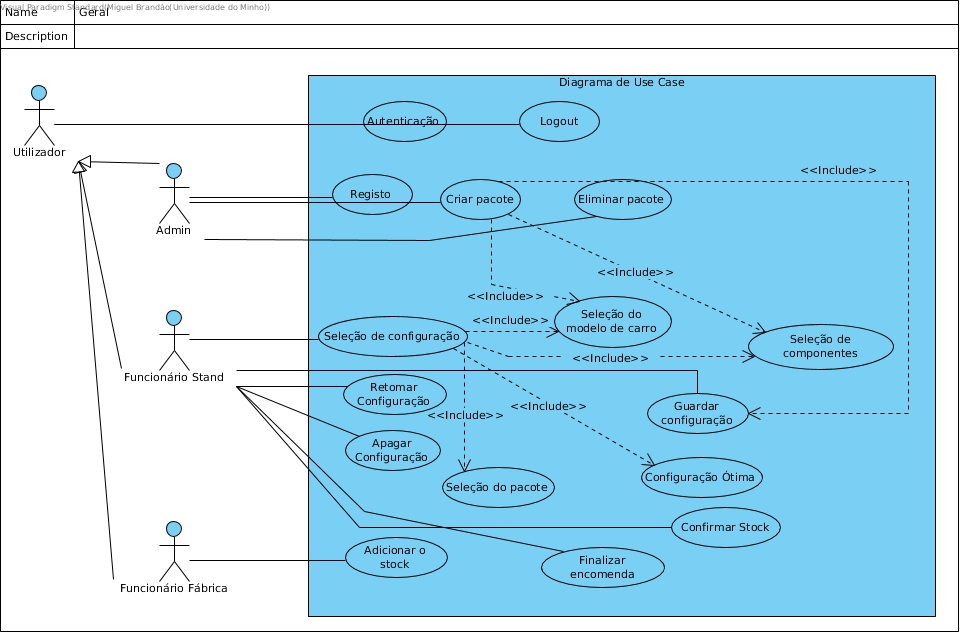
\includegraphics[width=\textwidth]{analise_de_requisitos/img/use_cases/diagrama_de_use_case.jpg}
    \caption{Diagrama de \textit{use cases}}
    \label{fig:diagrama_de_use_cases}
\end{figure}



Com o diagrama de \textit{use cases} representado pela figura \ref{fig:diagrama_de_use_cases}, podemos observar que temos 16 \textit{use cases} no total, sendo apenas dois deles comuns a todos os utilizadores (autenticação e \textit{logout}). Por vezes, foi necessário alterar os \textit{use cases}, conforme fomos construindo o programa e aumentando o nosso conhecimento do problema. Os \textit{use cases} estão especificados abaixo, com uma pequena descrição da sua função e uma referência para uma especificação no método tabular:
\begin{itemize}
    \item Autenticação (fig: \ref{fig:uc_autenticacao}): o utilizador entra no sistema;
    \item Logout (fig: \ref{fig:uc_logout}): o utilizador sai do sistema;
    \item Registo (fig: \ref{fig:uc_registo}): o administrador regista outro utilizador (quer seja funcionário de fábrica, funcionário de stand ou outro administrador);
    \item Criar Pacote (fig: \ref{fig:uc_criar_pacote}): o administrador cria um novo pacote de configuração que ainda não existe no sistema;
    \item Eliminar Pacote (fig: \ref{fig:uc_eliminar_pacote}): o administrador elimina um pacote de configuração existente no sistema;
    \item Retomar Configuração (fig: \ref{fig:uc_retormar_configuracao}): o funcionário de stand continua a configuração que tinha guardado anteriormente;
    \item Apagar Configuração (fig: \ref{fig:uc_apagar_configuracao}): o funcionário de stand apaga uma configuração guardada (se existir);
    \item Seleção de Configuração (fig: \ref{fig:uc_selecao_configuracao}):  o funcionário do stand cria uma nova configuração;
    \item Seleção do Modelo de Carro (fig: \ref{fig:uc_selecao_modelo_carro}): o funcionário de stand seleciona o tipo de carro que o cliente pretende encomendar;
    \item Seleção do Pacote (fig: \ref{fig:uc_selecao_pacote}): o funcionário de stand seleciona um pacote de configuração disponível a encomendar;
    \item Confirmar stock (fig: \ref{fig:uc_confirmar_stock}): a aplicação verifica se existe stock de todos os componentes pretendidos
    \item Configuração Ótima (fig: \ref{fig:uc_configuracao_otima}): o funcionário de stand insere o montante limite que o cliente está disposta a pagar e o sistema preenche automaticamente a melhor escolha;
    \item Seleção de Componentes (fig: \ref{fig:uc_selecao_componentes}): o funcionário de stand preenche manualmente cada componente para uma configuração personalizada;
    \item Guardar Configuração (fig: \ref{fig:uc_guardar_configuracao}): o funcionário de stand guarda a configuração do cliente no sistema para ser retomada no futuro;
   % \item Confirmar Encomenda: o funcionário de stand confirma que existe stock na fábrica para satisfazer a configuração do cliente;
    \item Finalizar Encomenda (fig: \ref{fig:uc_finalizar_encomenda}): o funcionário de stand finaliza a encomenda depois de ter sido confirmada (é enviada para a \textit{queue} de encomendas na fábrica);
    \item Adicionar o Stock (fig: \ref{fig:uc_adicionar_stock}): o funcionário de fábrica adiciona ou remove componentes manualmente no sistema.
\end{itemize}

\begin{figure}[ht]
    \centering
    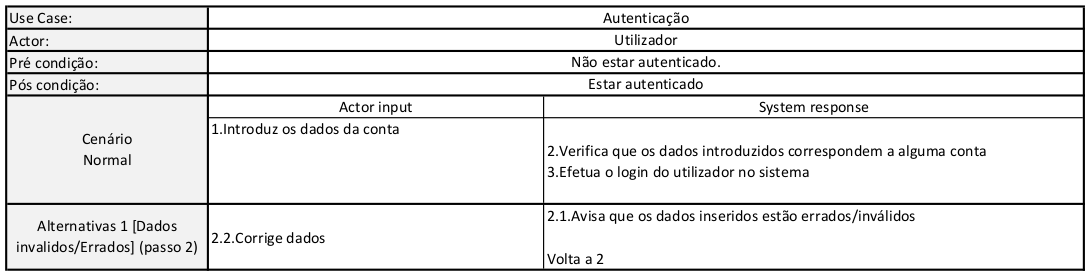
\includegraphics[width=\textwidth]{analise_de_requisitos/img/use_cases/autenticacao.png}
    \caption{\textit{Use case}: Autenticação}
    \label{fig:uc_autenticacao}
\end{figure}

\begin{figure}[ht]
    \centering
    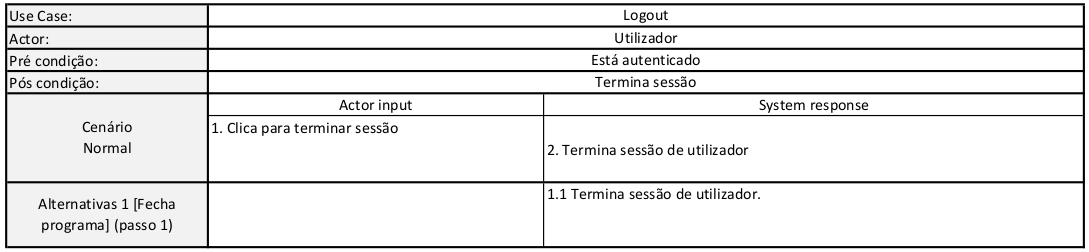
\includegraphics[width=\textwidth]{analise_de_requisitos/img/use_cases/logout.png}
    \caption{\textit{Use case}: Logout}
    \label{fig:uc_logout}
\end{figure}

\begin{figure}[ht]
    \centering
    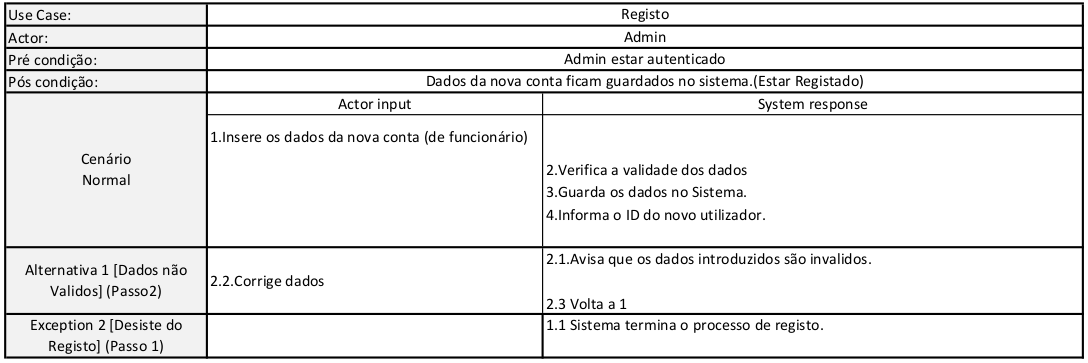
\includegraphics[width=\textwidth]{analise_de_requisitos/img/use_cases/registo.png}
    \caption{\textit{Use case}: Registo}
    \label{fig:uc_registo}
\end{figure}

\begin{figure}[ht]
    \centering
    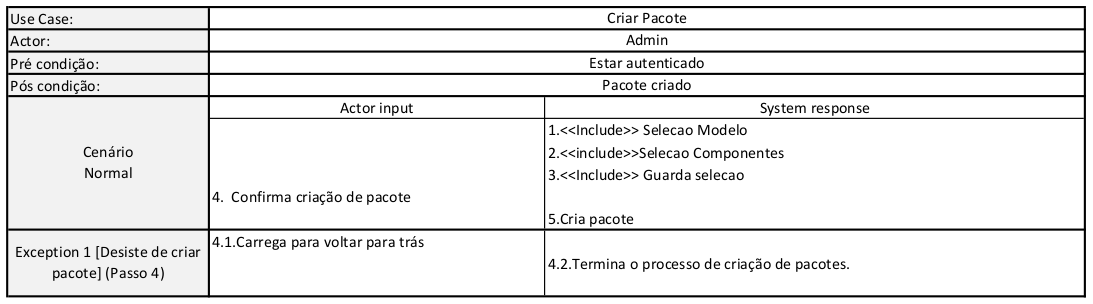
\includegraphics[width=\textwidth]{analise_de_requisitos/img/use_cases/criar_pacote.png}
    \caption{\textit{Use case}: Criar pacote}
    \label{fig:uc_criar_pacote}
\end{figure}

\begin{figure}[ht]
    \centering
    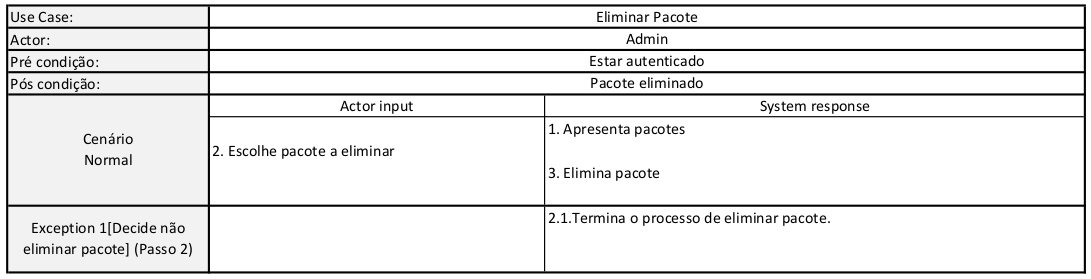
\includegraphics[width=\textwidth]{analise_de_requisitos/img/use_cases/eliminar_pacote.png}
    \caption{\textit{Use case}: Eliminar pacote}
    \label{fig:uc_eliminar_pacote}
\end{figure}

\begin{figure}[ht]
    \centering
    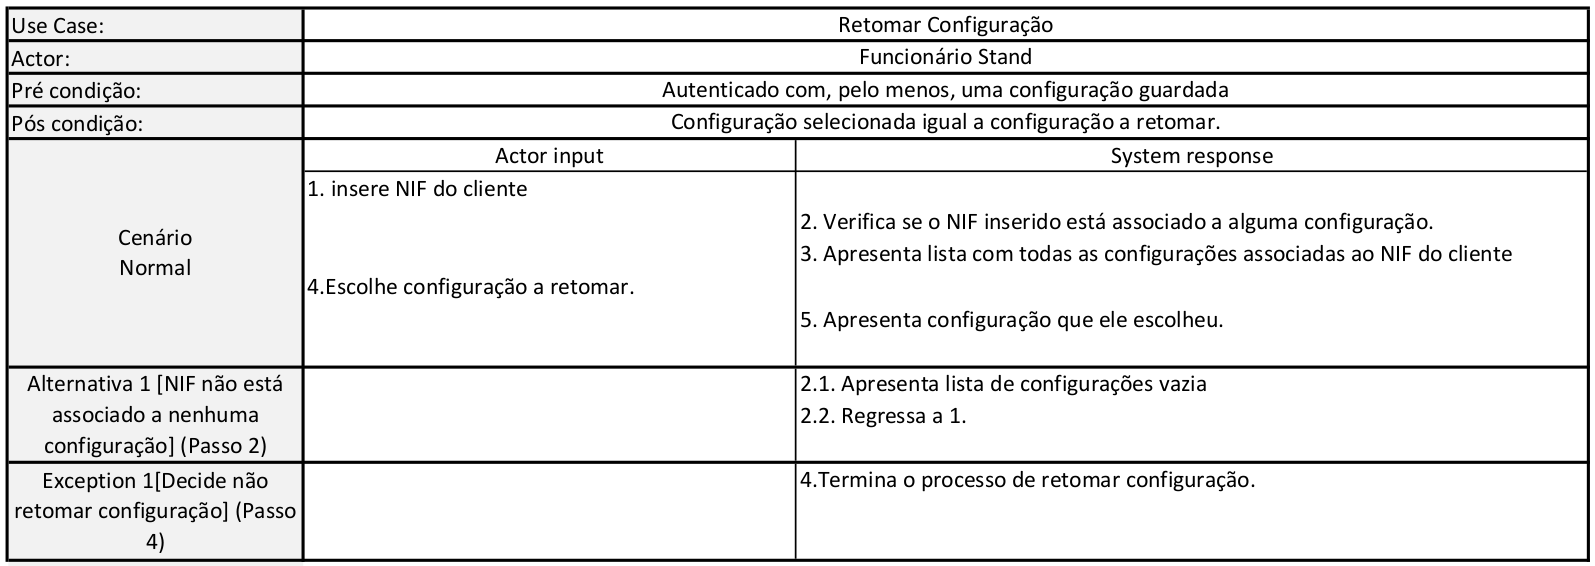
\includegraphics[width=\textwidth]{analise_de_requisitos/img/use_cases/retomar_configuracao.png}
    \caption{\textit{Use case}: Retomar configuração}
    \label{fig:uc_retormar_configuracao}
\end{figure}

\begin{figure}[ht]
    \centering
    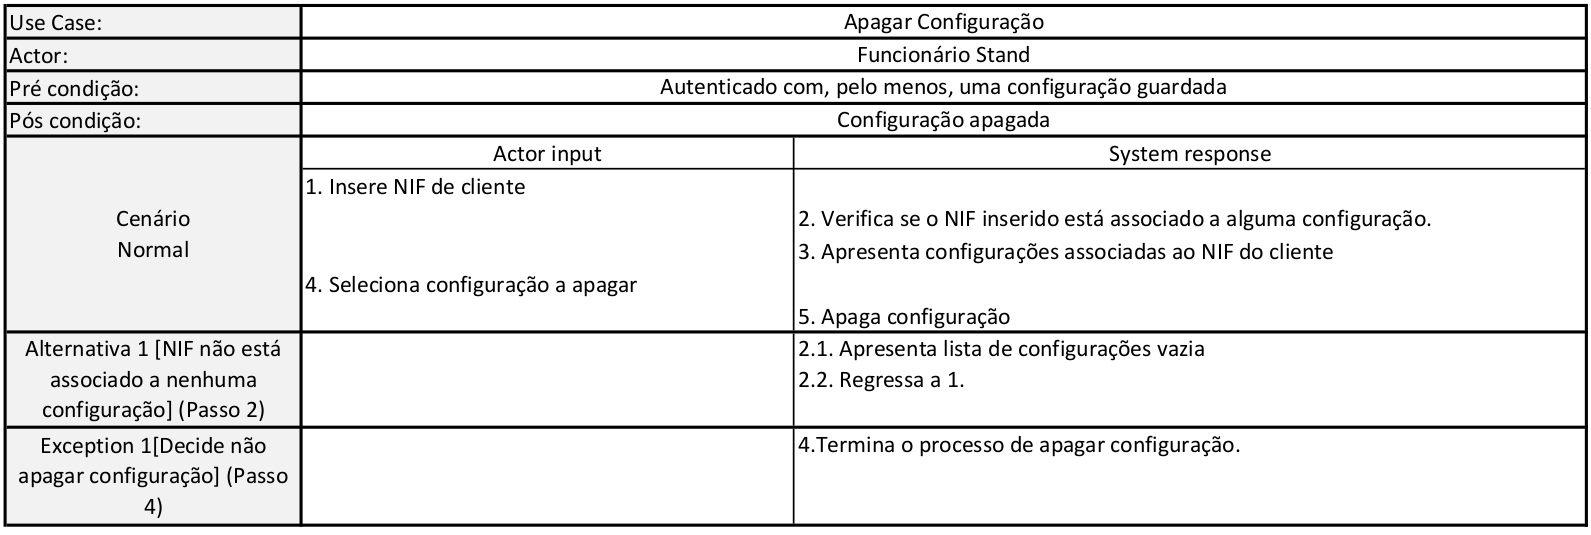
\includegraphics[width=\textwidth]{analise_de_requisitos/img/use_cases/apagar_configuracao.png}
    \caption{\textit{Use case}: Apagar configuração}
    \label{fig:uc_apagar_configuracao}
\end{figure}

\begin{figure}[ht]
    \centering
    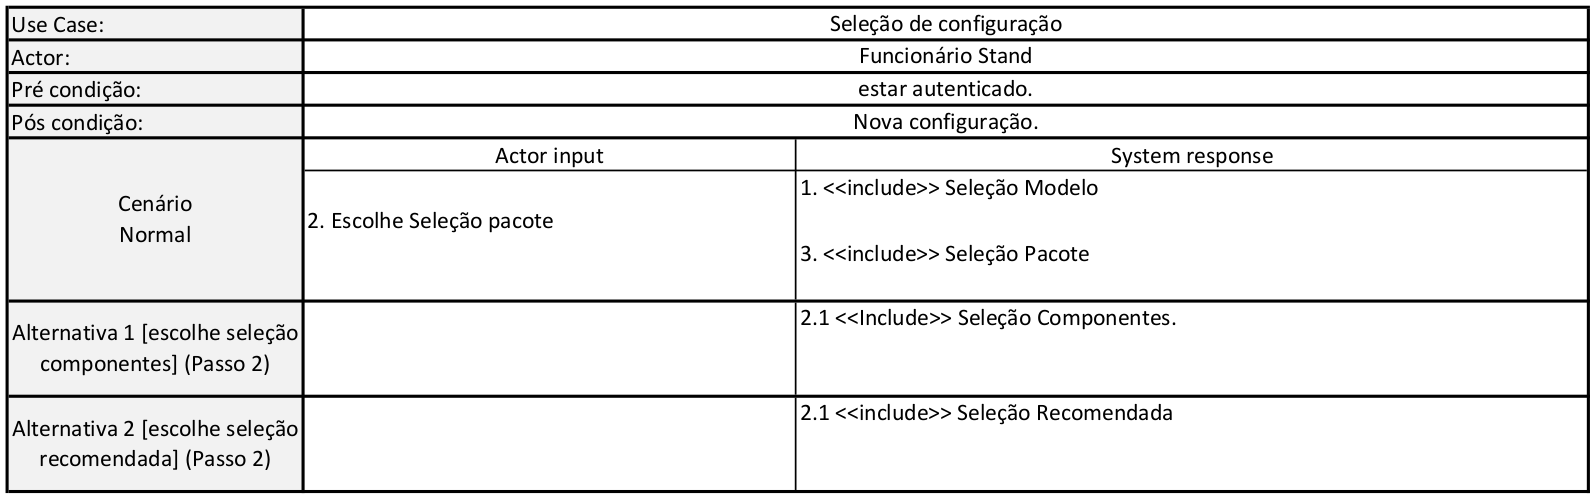
\includegraphics[width=\textwidth]{analise_de_requisitos/img/use_cases/selecao_configuracao.png}
    \caption{\textit{Use case}: Seleção de configuração}
    \label{fig:uc_selecao_configuracao}
\end{figure}

\begin{figure}[ht]
    \centering
    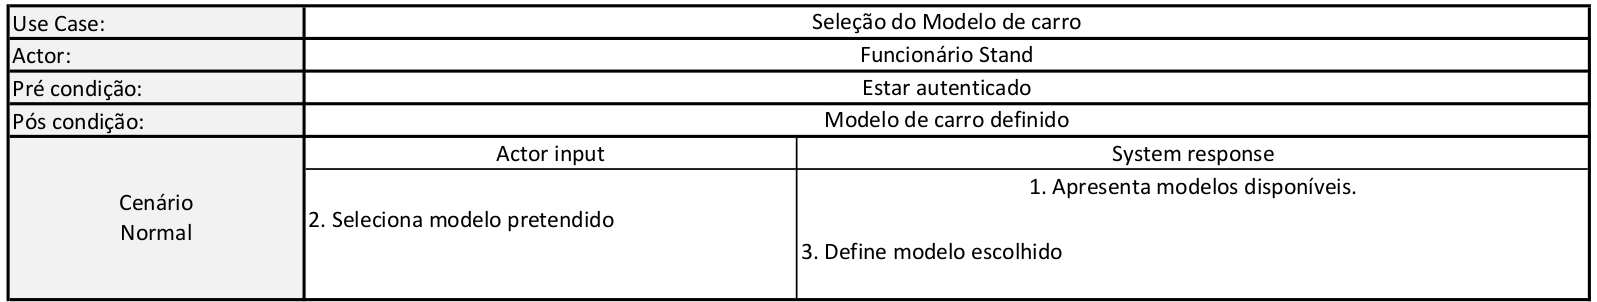
\includegraphics[width=\textwidth]{analise_de_requisitos/img/use_cases/selecao_modelo_carro.png}
    \caption{\textit{Use case}: Seleção do Modelo de Carro}
    \label{fig:uc_selecao_modelo_carro}
\end{figure}

\begin{figure}[ht]
    \centering
    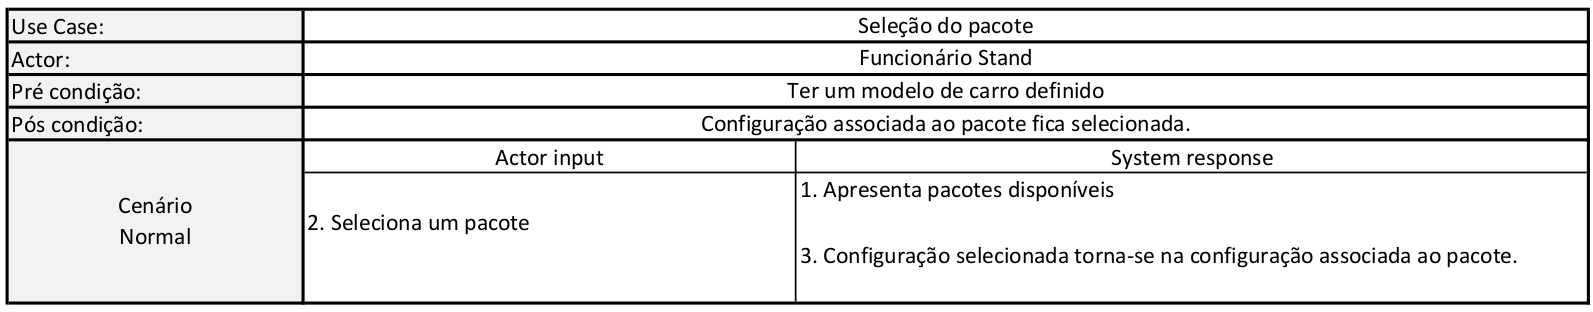
\includegraphics[width=\textwidth]{analise_de_requisitos/img/use_cases/selecao_pacote.png}
    \caption{\textit{Use case}: Seleção do pacote}
    \label{fig:uc_selecao_pacote}
\end{figure}

\begin{figure}[ht]
    \centering
    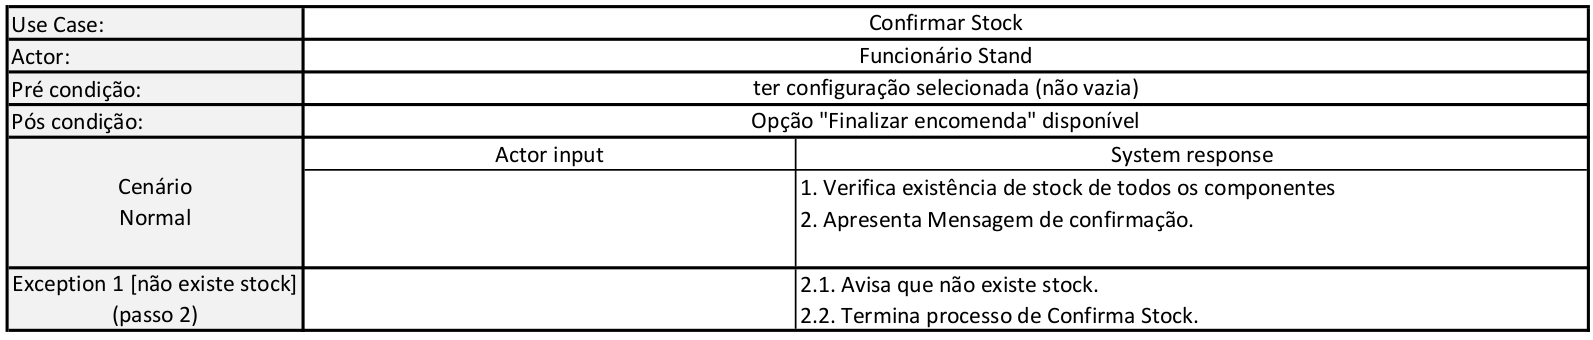
\includegraphics[width=\textwidth]{analise_de_requisitos/img/use_cases/confirmar_stock.png}
    \caption{\textit{Use case}: Confirmar Stock}
    \label{fig:uc_confirmar_stock}
\end{figure}

\begin{figure}[ht]
    \centering
    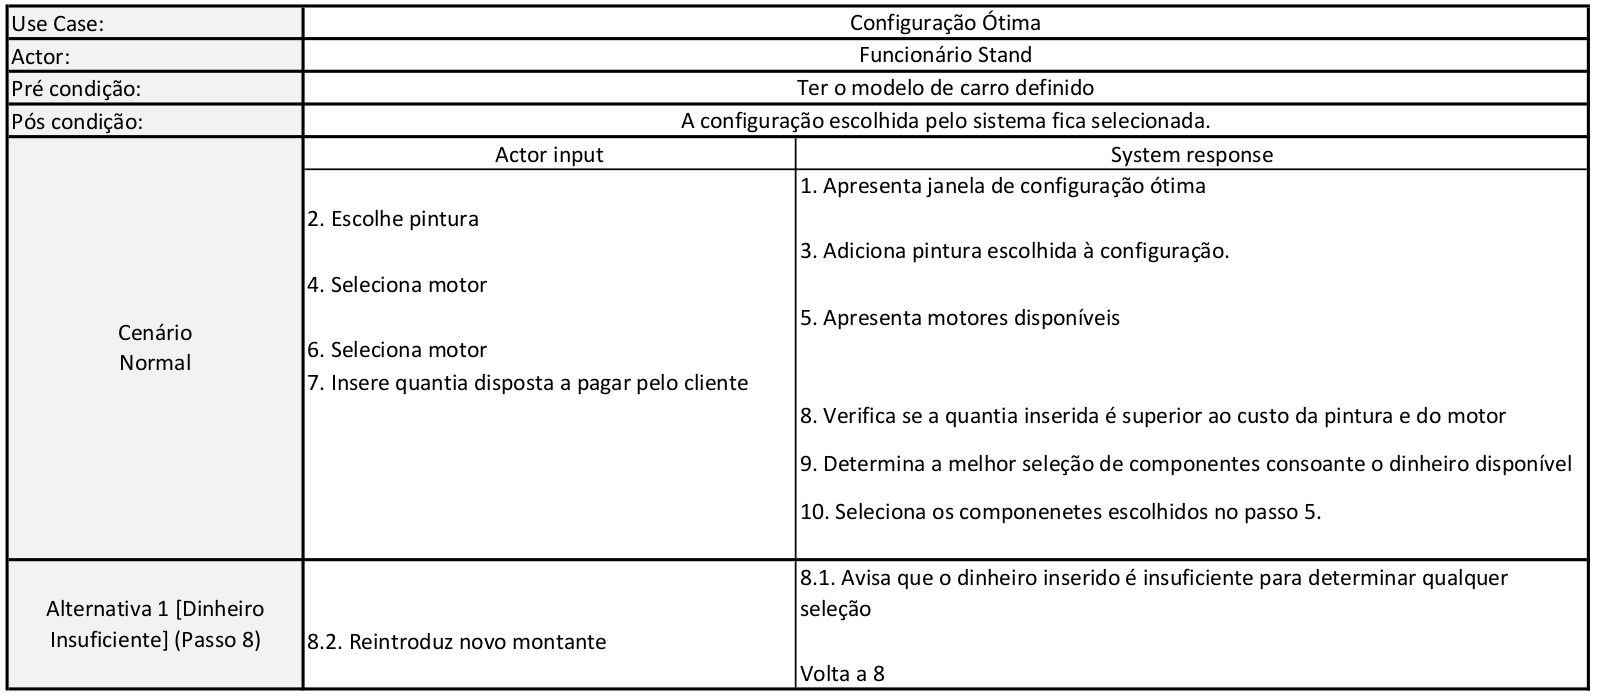
\includegraphics[width=\textwidth]{analise_de_requisitos/img/use_cases/configuracao_otima.png}
    \caption{\textit{Use case}: Configuração Ótima}
    \label{fig:uc_configuracao_otima}
\end{figure}

\begin{figure}[ht]
    \centering
    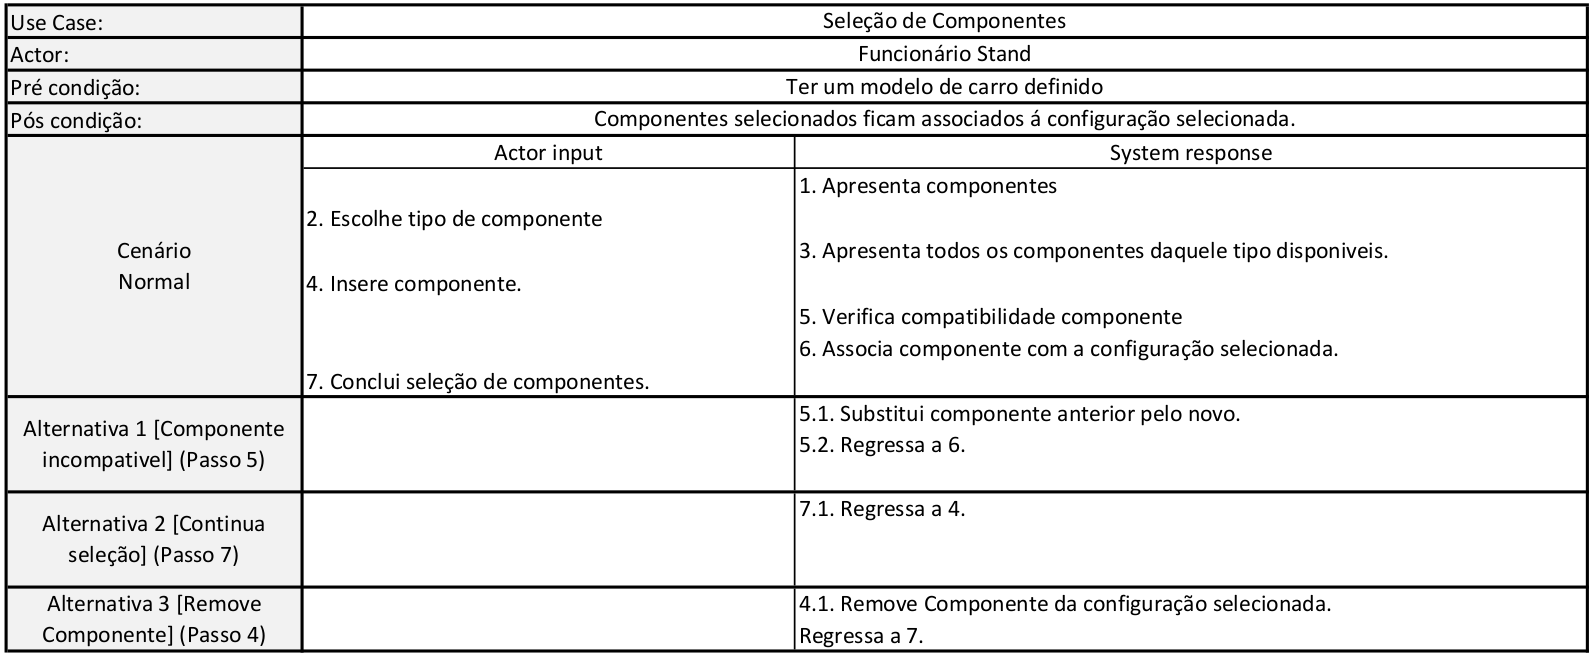
\includegraphics[width=\textwidth]{analise_de_requisitos/img/use_cases/selecao_componentes.png}
    \caption{\textit{Use case}: Seleção de Componentes}
    \label{fig:uc_selecao_componentes}
\end{figure}

\begin{figure}[ht]
    \centering
    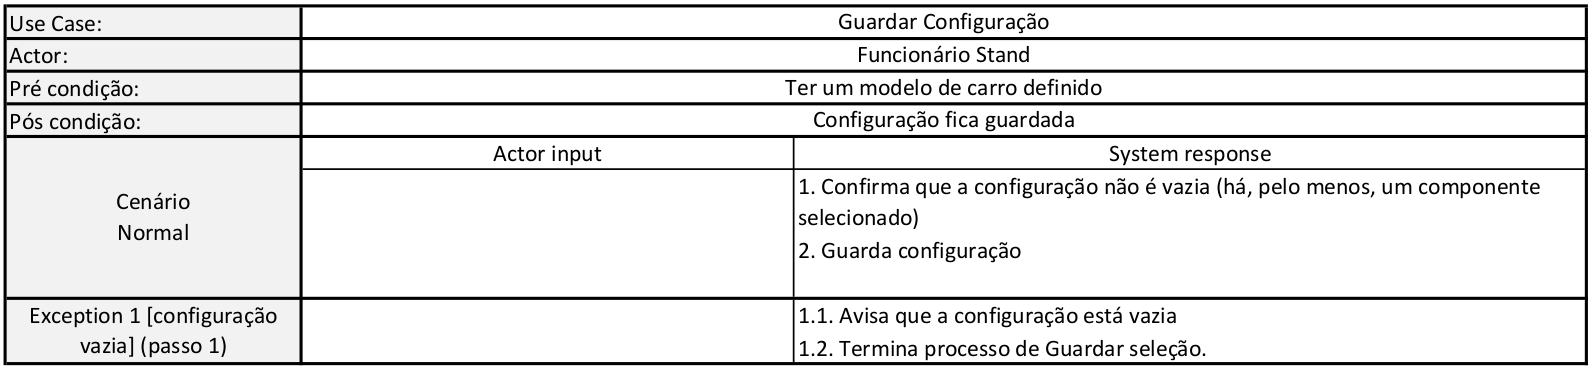
\includegraphics[width=\textwidth]{analise_de_requisitos/img/use_cases/guardar_configuracao.png}
    \caption{\textit{Use case}: Guardar Configuração}
    \label{fig:uc_guardar_configuracao}
\end{figure}

\begin{figure}[ht]
    \centering
    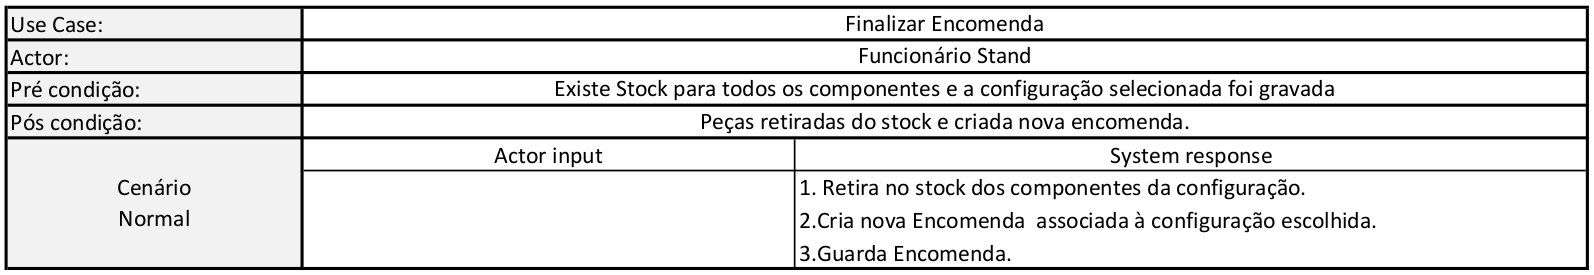
\includegraphics[width=\textwidth]{analise_de_requisitos/img/use_cases/finalizar_encomenda.png}
    \caption{\textit{Use case}: Finalizar Encomenda}
    \label{fig:uc_finalizar_encomenda}
\end{figure}

\begin{figure}[ht]
    \centering
    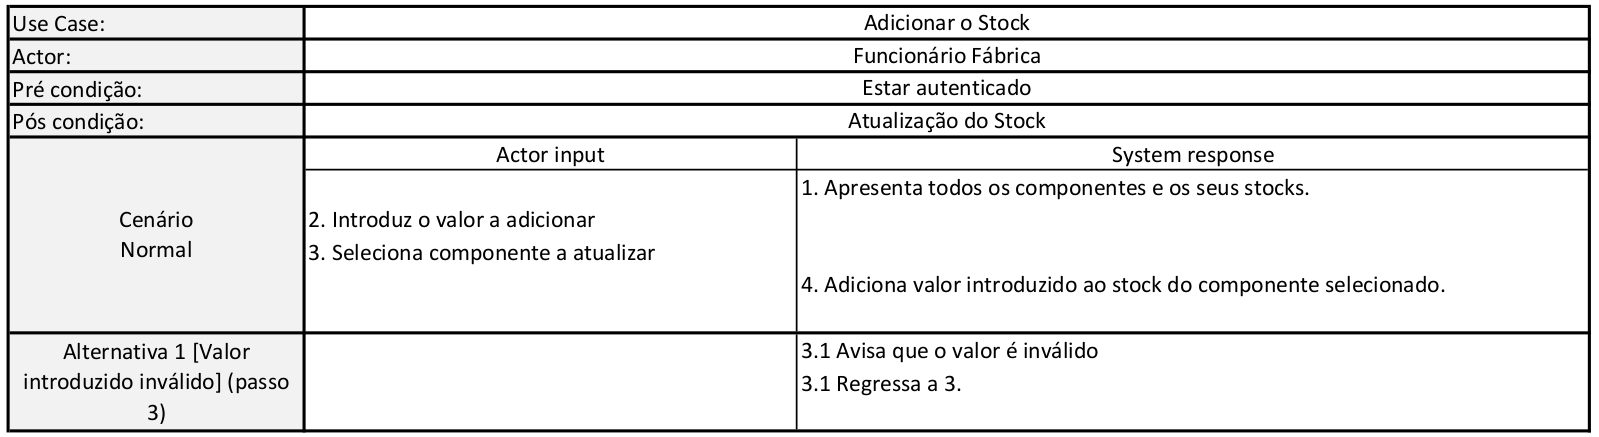
\includegraphics[width=\textwidth]{analise_de_requisitos/img/use_cases/adicionar_stock.png}
    \caption{\textit{Use case}: Adicionar o Stock}
    \label{fig:uc_adicionar_stock}
\end{figure}

\clearpage